\section{外推一：加勒比海}\label{sec:carib}

\subsection{选点标准与结果}

为了检验模型的可迁移性，我们按同一套标准在加勒比海选点：\emph{距小岛不远、
4$\times$4 km 内水深与主算例可比、地形复杂、海况（流场）更复杂}。
最终选定\textbf{小开曼岛（Little Cayman）西南、开曼海槽边缘}：
失事海域中心 19.6076°N、80.1868°W，出发点为小开曼岛西端
（19.6521°N、80.1229°W，距失事点 8.3 km）。

\begin{table}[H]
\centering\small
\caption{两个海域的环境对比}
\label{tab:twoseas}
\begin{tabular}{@{}lcc@{}}
\toprule
指标 & 地中海（主算例） & 加勒比海（外推）\\
\midrule
失事点当地海底深度（10/50/90\%） & 574/1021/1607 m & 880/1034/1492 m\\
失事点海底坡度（中位/90\%） & 16.9° / 23.3° & 15.1° / 22.1°\\
表层流速（剖面平均） & 0.22 m/s & \textbf{0.47 m/s}\\
100 m 层流速（4D，90\% 分位） & 0.23 m/s & \textbf{0.56 m/s}\\
300 m 层流速（4D，90\% 分位） & 0.044 m/s & 0.025 m/s\\
96 h 漂移（中位/90\% 分位） & 23.7 / 93.2 km & \textbf{58.6 / 191.8 km}\\
沉底分支终点深度（中位） & 1442 m & 1073 m\\
水柱/海底/水面终态占比 & 62/16/22\% & 62/15/22\%\\
\bottomrule
\end{tabular}
\end{table}

\begin{figure}[H]
\centering
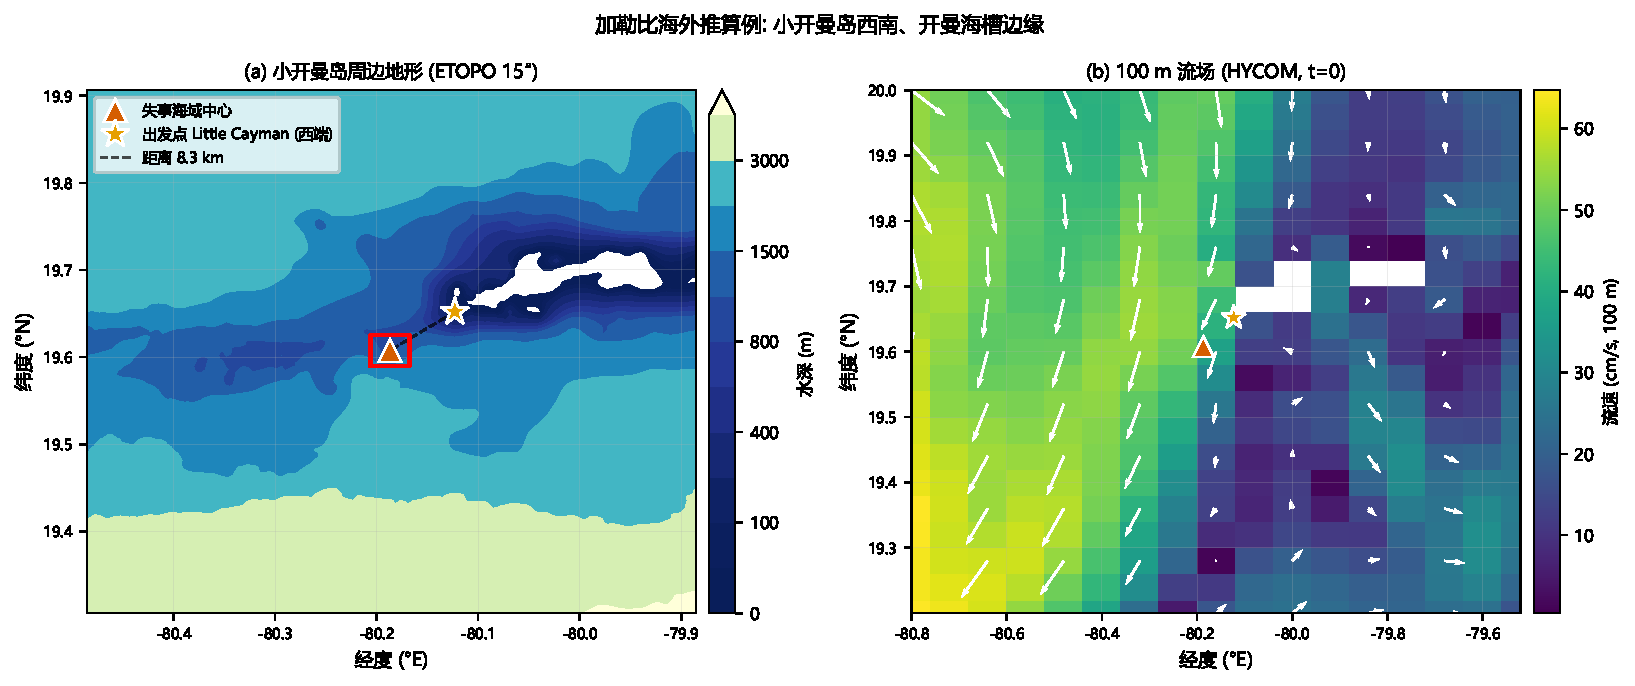
\includegraphics[width=0.76\textwidth]{fig_carib_map}
\caption{加勒比海算例。(a) 小开曼岛周边地形与 4$\times$4 km 失事海域、出发点；
(b) 100 m 层 HYCOM 流场（t=0），可见明显的空间梯度与涡旋结构。}
\label{fig:carib-map}
\end{figure}

\begin{figure}[H]
\centering
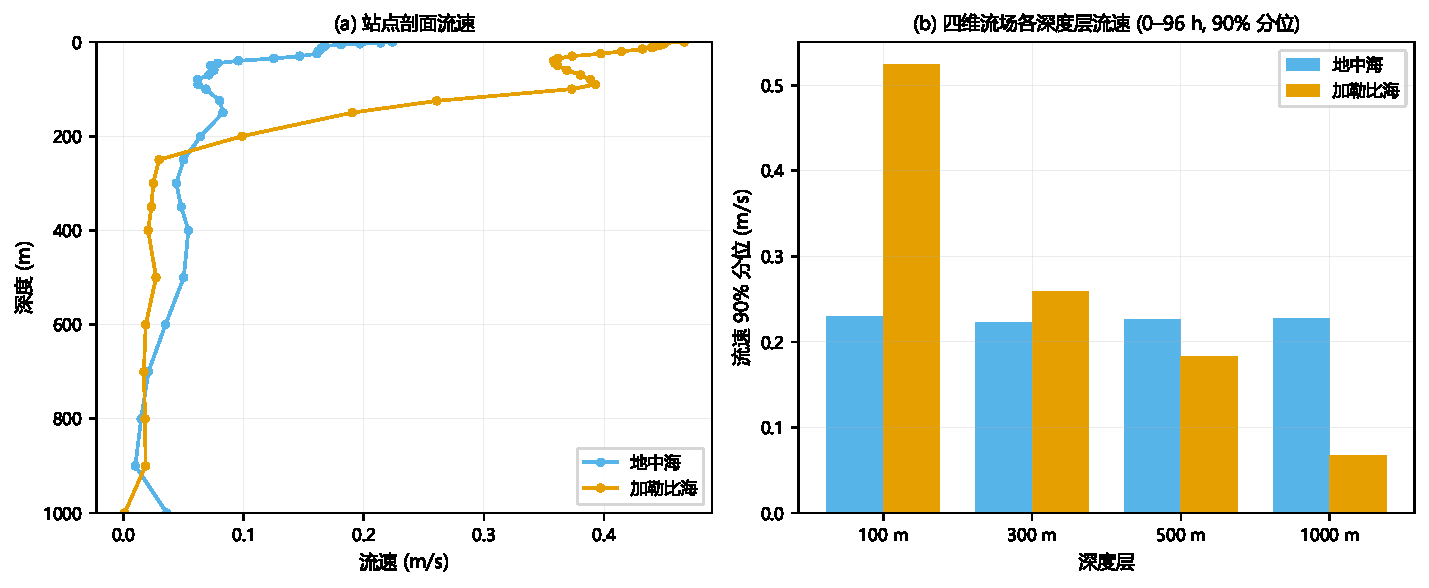
\includegraphics[width=0.72\textwidth]{fig_carib_current}
\caption{两个海域的流场对比：(a) 站点剖面流速（加勒比海 0--200 m 明显更强）；
(b) 四维流场各深度层 90\% 分位流速（加勒比海 100 m 层约为地中海的 2.4 倍，
但 500--1000 m 层反而更弱）。}
\label{fig:carib-current}
\end{figure}

\subsection{结果：成功率几乎不变}

用完全相同的模型（30\,000 粒子、7 种装备组合、相同的探测与协调参数）重跑，
7 种单船组合的 $P_{72}$ 与主算例几乎相同（\tabref{tab:carib-schemes}）。

\begin{table}[H]
\centering\small
\caption{7 种单船组合的 $P_{72}$：两个海域对比}
\label{tab:carib-schemes}
\begin{tabular}{@{}llccc@{}}
\toprule
编号 & 组合 & 地中海 & 加勒比海 & 差值\\
\midrule
M1 & 侧扫 & 38.2\% & 36.9\% & $-1.3$\\
M2 & 多波束 & 86.5\% & 86.8\% & $+0.3$\\
M3 & AUV & 78.9\% & 81.3\% & $+2.4$\\
M4 & 侧扫+多波束 & 89.6\% & 89.7\% & $+0.1$\\
M5 & 侧扫+AUV & 84.5\% & 85.9\% & $+1.4$\\
M6 & 多波束+AUV & 94.3\% & 94.3\% & $0.0$\\
M7 & 侧扫+多波束+AUV & 95.5\% & 95.6\% & $+0.1$\\
\bottomrule
\end{tabular}
\end{table}

\begin{figure}[H]
\centering
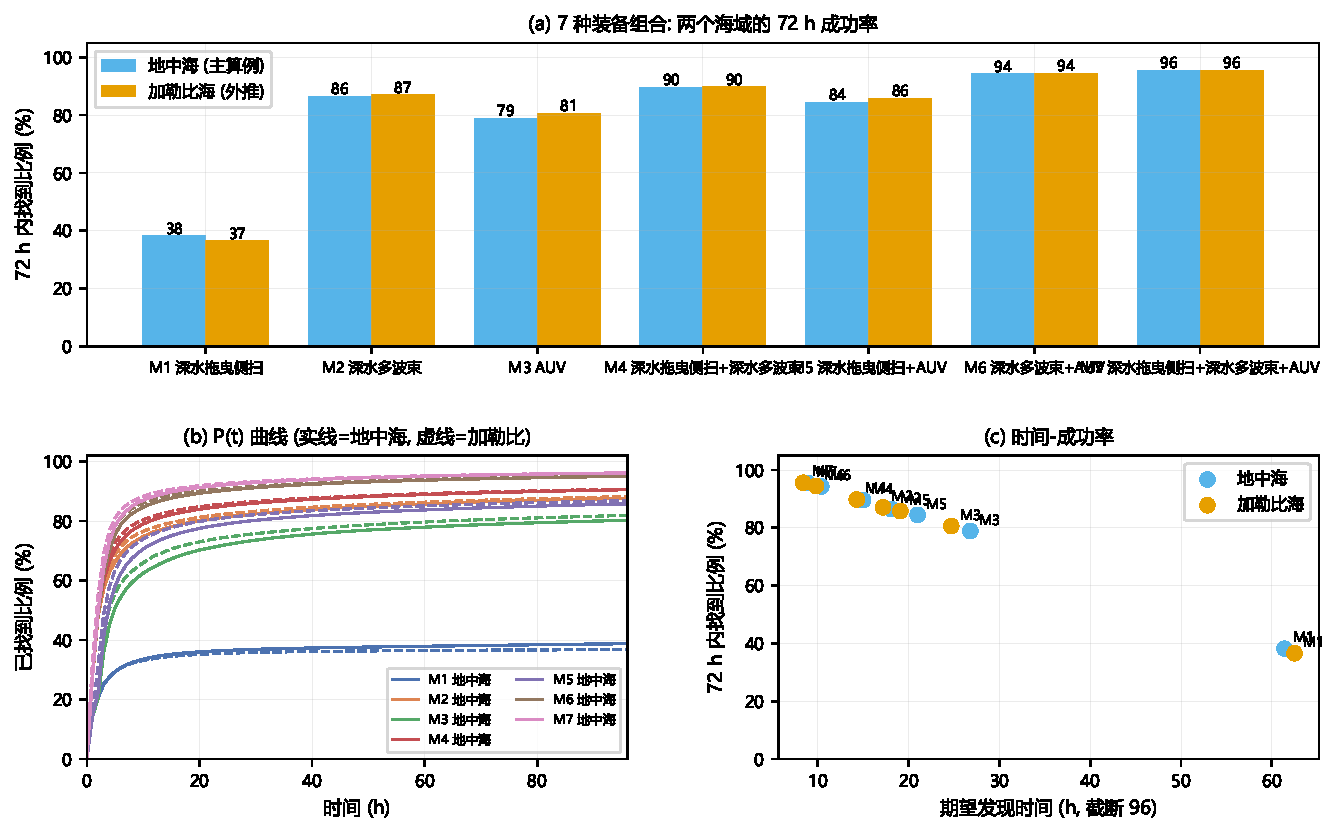
\includegraphics[width=0.76\textwidth]{fig_carib_compare}
\caption{两个海域的搜索结果对比：(a) 7 种方案的 $P_{72}$ 柱状图；
(b) 全部 $P(t)$ 曲线（实线地中海、虚线加勒比海）；(c) 时间–成功率散点。
方案排序与结论完全一致。}
\label{fig:carib-compare}
\end{figure}

15 种多船组合的结论也一致：2 船 96.2\%、2 船+2 AUV 98.7\%、4 船+4 AUV 99.8\%，
与主算例的 96.6\%/98.9\%/99.9\% 相差不到 1 个百分点；“先加船、后加 AUV”的边际效益
规律相同。

\subsection{为什么“漂移大 2.5 倍，成功率几乎不变”？}

\begin{enumerate}[leftmargin=1.8em,itemsep=0pt]
\item \textbf{搜索方的预测云跟着流场走}：30\,000 个粒子的漂移由同一套四维流场驱动，
      预测云与真实云同步平移；只要预报准确，目标的绝对漂移距离不直接增加搜索难度，
      真正决定难度的是\emph{预测云的相对离散度}与装备的覆盖能力；
\item \textbf{加勒比海的大漂移主要来自表层分支}（0.47 m/s）：水面目标由雷达/目视搜索
      （扫宽 3 km），大漂移对它的影响很小；水柱与沉底分支在 300 m 以深流速反而与
      地中海相当甚至更弱（\figref{fig:carib-current}b）；
\item 因此两个海域的“位置不确定性增长率”相近（\figref{fig:carib-drift}），
      搜索成功率自然相近。
\end{enumerate}

\begin{figure}[H]
\centering
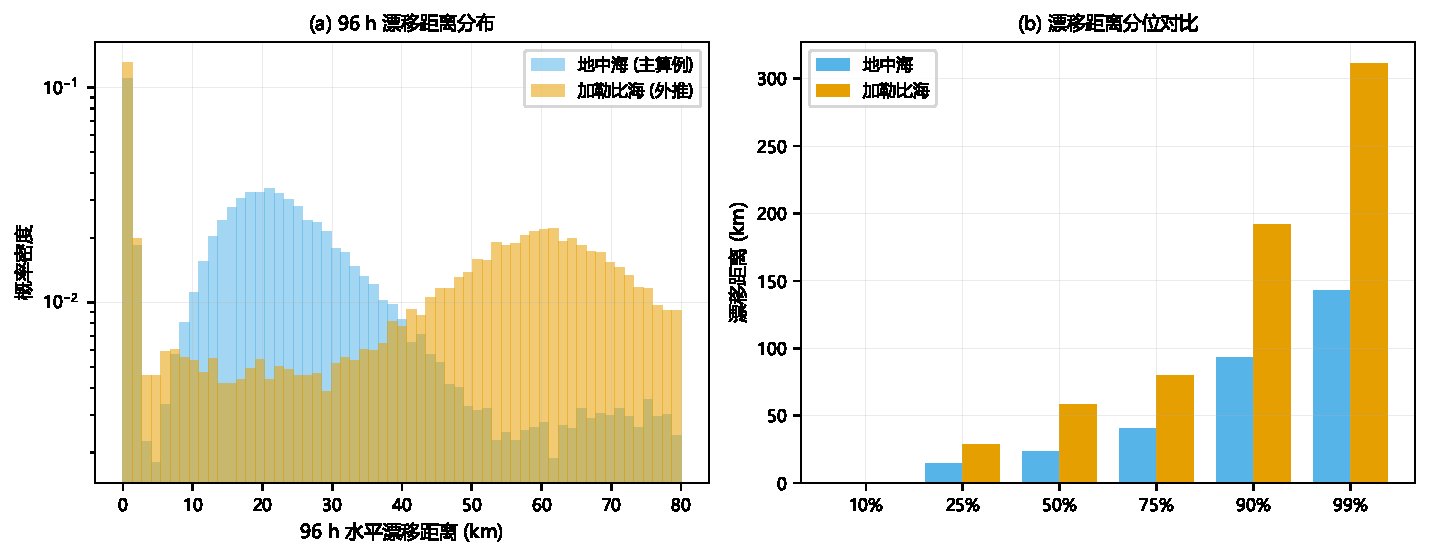
\includegraphics[width=0.84\textwidth]{fig_carib_drift}
\caption{两个海域的 96 h 漂移距离分布（a）与分位对比（b）。加勒比海的漂移中位数约为
地中海的 2.5 倍，但主要由表面分支贡献。}
\label{fig:carib-drift}
\end{figure}



\subsection{重要限定}

本模型采用\textbf{完美预报}假设（预测与真值用同一套流场），因此会\emph{低估}
复杂海况的实际难度：加勒比海表层流速大、涡旋多，真实预报误差显著大于地中海，
实际成功率会低于本文结果。这一局限性恰好给出运营建议：
对强流/涡旋海域，不能照搬地中海的配置，而应同时加强
（1）现场流场观测与预报订正、（2）冗余能力（多 1 艘船或 2 台 AUV）。
换言之，\textbf{“漂移大”不可怕，“预报不准”才可怕}。
